% MIT Thesis Proposal Template
% Created by Micah Smith <micahs@mit.edu>
% link: https://github.com/mit-eecs-gsa/mit-eecs-thesis-proposal-template/tree/master#

\documentclass{article}

\usepackage{geometry}
\usepackage{parskip}
\usepackage{graphicx}
\usepackage{subcaption}
\usepackage{xcolor}

% must be last in usepackage list!
\usepackage{hyperref}
\usepackage{cleveref}


% other stuff
\newcommand\hmng[1]{\textcolor{blue!40!red}{[hmng: {#1}]}}
\newcommand{\mydate}{August 2025}
\newcommand{\mycompletion}{September 2025}
\newcommand{\mytitle}{Modifying Linux to separate best effort from latency critical workloads}

\newcommand{\schedidle}{\texttt{sched\_idle}}
\newcommand{\schednormal}{\texttt{sched\_normal}}

\author{
    Hannah Manuela Nelle Gross\\
    Massachusetts Institute of Technology\\
    \texttt{hannah@csail.mit.edu}
}

\date{\mydate}

\title{\mytitle}

\begin{document}

% MIT S.M. Thesis Proposal Title Page Template
% Created by Micah Smith
% This is based off of the thesis proposal title page shown in "Thesis Proposal and Thesis
% Guidelines 2015.pdf", distributed by the MIT EECS Graduate Office.

\begingroup
\fontfamily{phv}\large\selectfont

\newgeometry{left=1in,right=1in}

\begin{center}
Massachusetts Institute of Technology \\
Department of Electrical Engineering and Computer Science
\end{center}

\begin{center}
Proposal for Thesis Research in Partial Fulfillment \\
of the Requirements for the Degree of \\
Master of Science
\end{center}

\vspace{1em}
\noindent Title: \mytitle

\vspace{1em}
\noindent\begin{tabular}{@{}ll}
Submitted by: & Hannah Gross\\
              & 32 Vassar St \\
              & Cambridge, MA 02139
\end{tabular}

\vspace{1em}
\noindent Signature of author: \rule{5cm}{0.1pt}

\vspace{1em}
\noindent Date of Submission: \mydate

\vspace{1em}
\noindent Expected Date of Completion: \mycompletion

\vspace{1em}
\noindent Laboratory: PDOS

\vspace{1em}
\noindent Brief Statement of the Problem:

\vspace{1em}
\begin{minipage}{\dimexpr\textwidth-1cm}

\noindent Many popular containerization framekworks rely on Linux's cgroups to
isolate the performance of latency critical containers from best effort ones
running on the same machine. This thesis shows that Linux's current mechanism,
based on weights, is unable to do so. We make the split explicit by putting best
effort work in a separate scheduling class, and show that this improves Linux's
ability to isolate.

\end{minipage}

\vspace{1em}
\noindent Supervision Agreement:

\vspace{1em}
\begin{minipage}{\dimexpr\textwidth-1cm}
\noindent The program outlined in this proposal is adequate for a Master's thesis. The
supplies and facilities required are available, and I am willing to supervise
the research and evaluate the thesis report.
\end{minipage}

\vspace{2em}
\begin{flushright}
    \rule{0.7\linewidth}{0.1pt}\\
    {\normalsize Your Advisor, Their Title}
\end{flushright}

\restoregeometry

\endgroup


\newpage

\maketitle

\begin{abstract}
    
Widely-used container orchestration systems like Kubernetes are surprisingly
unable to honor the reservations of LC applications in the presence BE
workloads: a Kubernetes web application's mean latency jumps from 6.2ms to
$\sim$13ms after starting a BE image resize job. This paper traces this problem
down to Linux's cgroups, and show that because Linux uses per-core runqueues,
its weight-based interface is not enforced across cores.

This paper proposes an API that separates best effort workloads from critical
ones with reservations by introducing the BeClass priority class. BeClass
requires fewer cross-core interactions than a weight-based approach, and ensures
that no BE is ever running when an LC is queued. During high load this requires
`parking', which enforces that BEs user-space code doesn't run if doing so would
interrupt an LC process, but continues to run kernel-level services for the BE
so that when load goes down it can continue to run.

Experiments with a BeClass implementation in Linux show that BeClass ensures LC
processes' access to their reserved cores, while running BE workloads
opportunistically. When using BeClass in the same Kubernetes experiment, the
application's mean latency stayed stable at 6.2ms even after starting the BE.

\end{abstract}


%-------------------------------------------------------------------------------
\section{Introduction}
\label{s:intro}
%-------------------------------------------------------------------------------

Cloud providers like AWS and Google, as well as deployment management systems
like Kubernetes, allow users to run services by attaching to each an amount of
resources the service will get. This includes compute (a number of vCPUs),
memory, and sometimes network bandwidth~\cite{aws-ec2-resources,
kubernetes-resources}; the resource this work focuses on is CPU. The guarantee
developers get is that the service will have undisturbed access to that amount
of resources.

Enforcing this guanatee is hard. If providers leave the CPUs idle so they are
available when the service needs them, that leads to a utilization problem. The
load on most applications run in the cloud is variable and unpredictable, so to
account for this developers choose the amount of resources to reserve based on
the expected peak load~\cite{borg, nu, overprovision}. This means that services
with reserved resources rarely use the full reservation they asked for. 

What most systems do instead is allow other workloads to run opportunistically
on temporarly unutilized resources. This includes so-called \textit{best effort}
workloads, which have no reservations, as well letting services with
reservations temporarily \textit{burst}, meaning use more CPUs than they asked
for. This solves the utilization problem, without requiring compromises on the
guarantees made: services with reservations get access to the CPUs they
requested when desired, while best effort or bursting services can make use of
otherwise idle resources.

Kubernetes follows presicely this model. Services fall into three quality of
service (QOS) classes: \textit{Guaranteed}, which have requests (\ie{}
reservations) as well as limits, \textit{Burstable}, which have requests and no
limits, and \textit{Best Effort}, which have
neither~\cite{kubernetes-pod-qos-types}. Guaranteed services are the last to be
evicted from a node experiencing high load, and give more predictable
performance, whereas the Burstable class allows applications with bursty load to
opportunistically make use of available resources, thereby better utilizing the
resources Kubernetes is running on.

AWS similarly supports both guaranteed- and burstable-style reservations, with
their M and T instance types~\cite{aws-ec2-burstable,aws-ec2-resources}. In this
case the motivation for customers to use the burstable-style instance rather
than overprovisioning on guaranteed-style is pricing.


\begin{figure}[t]
    \centering
    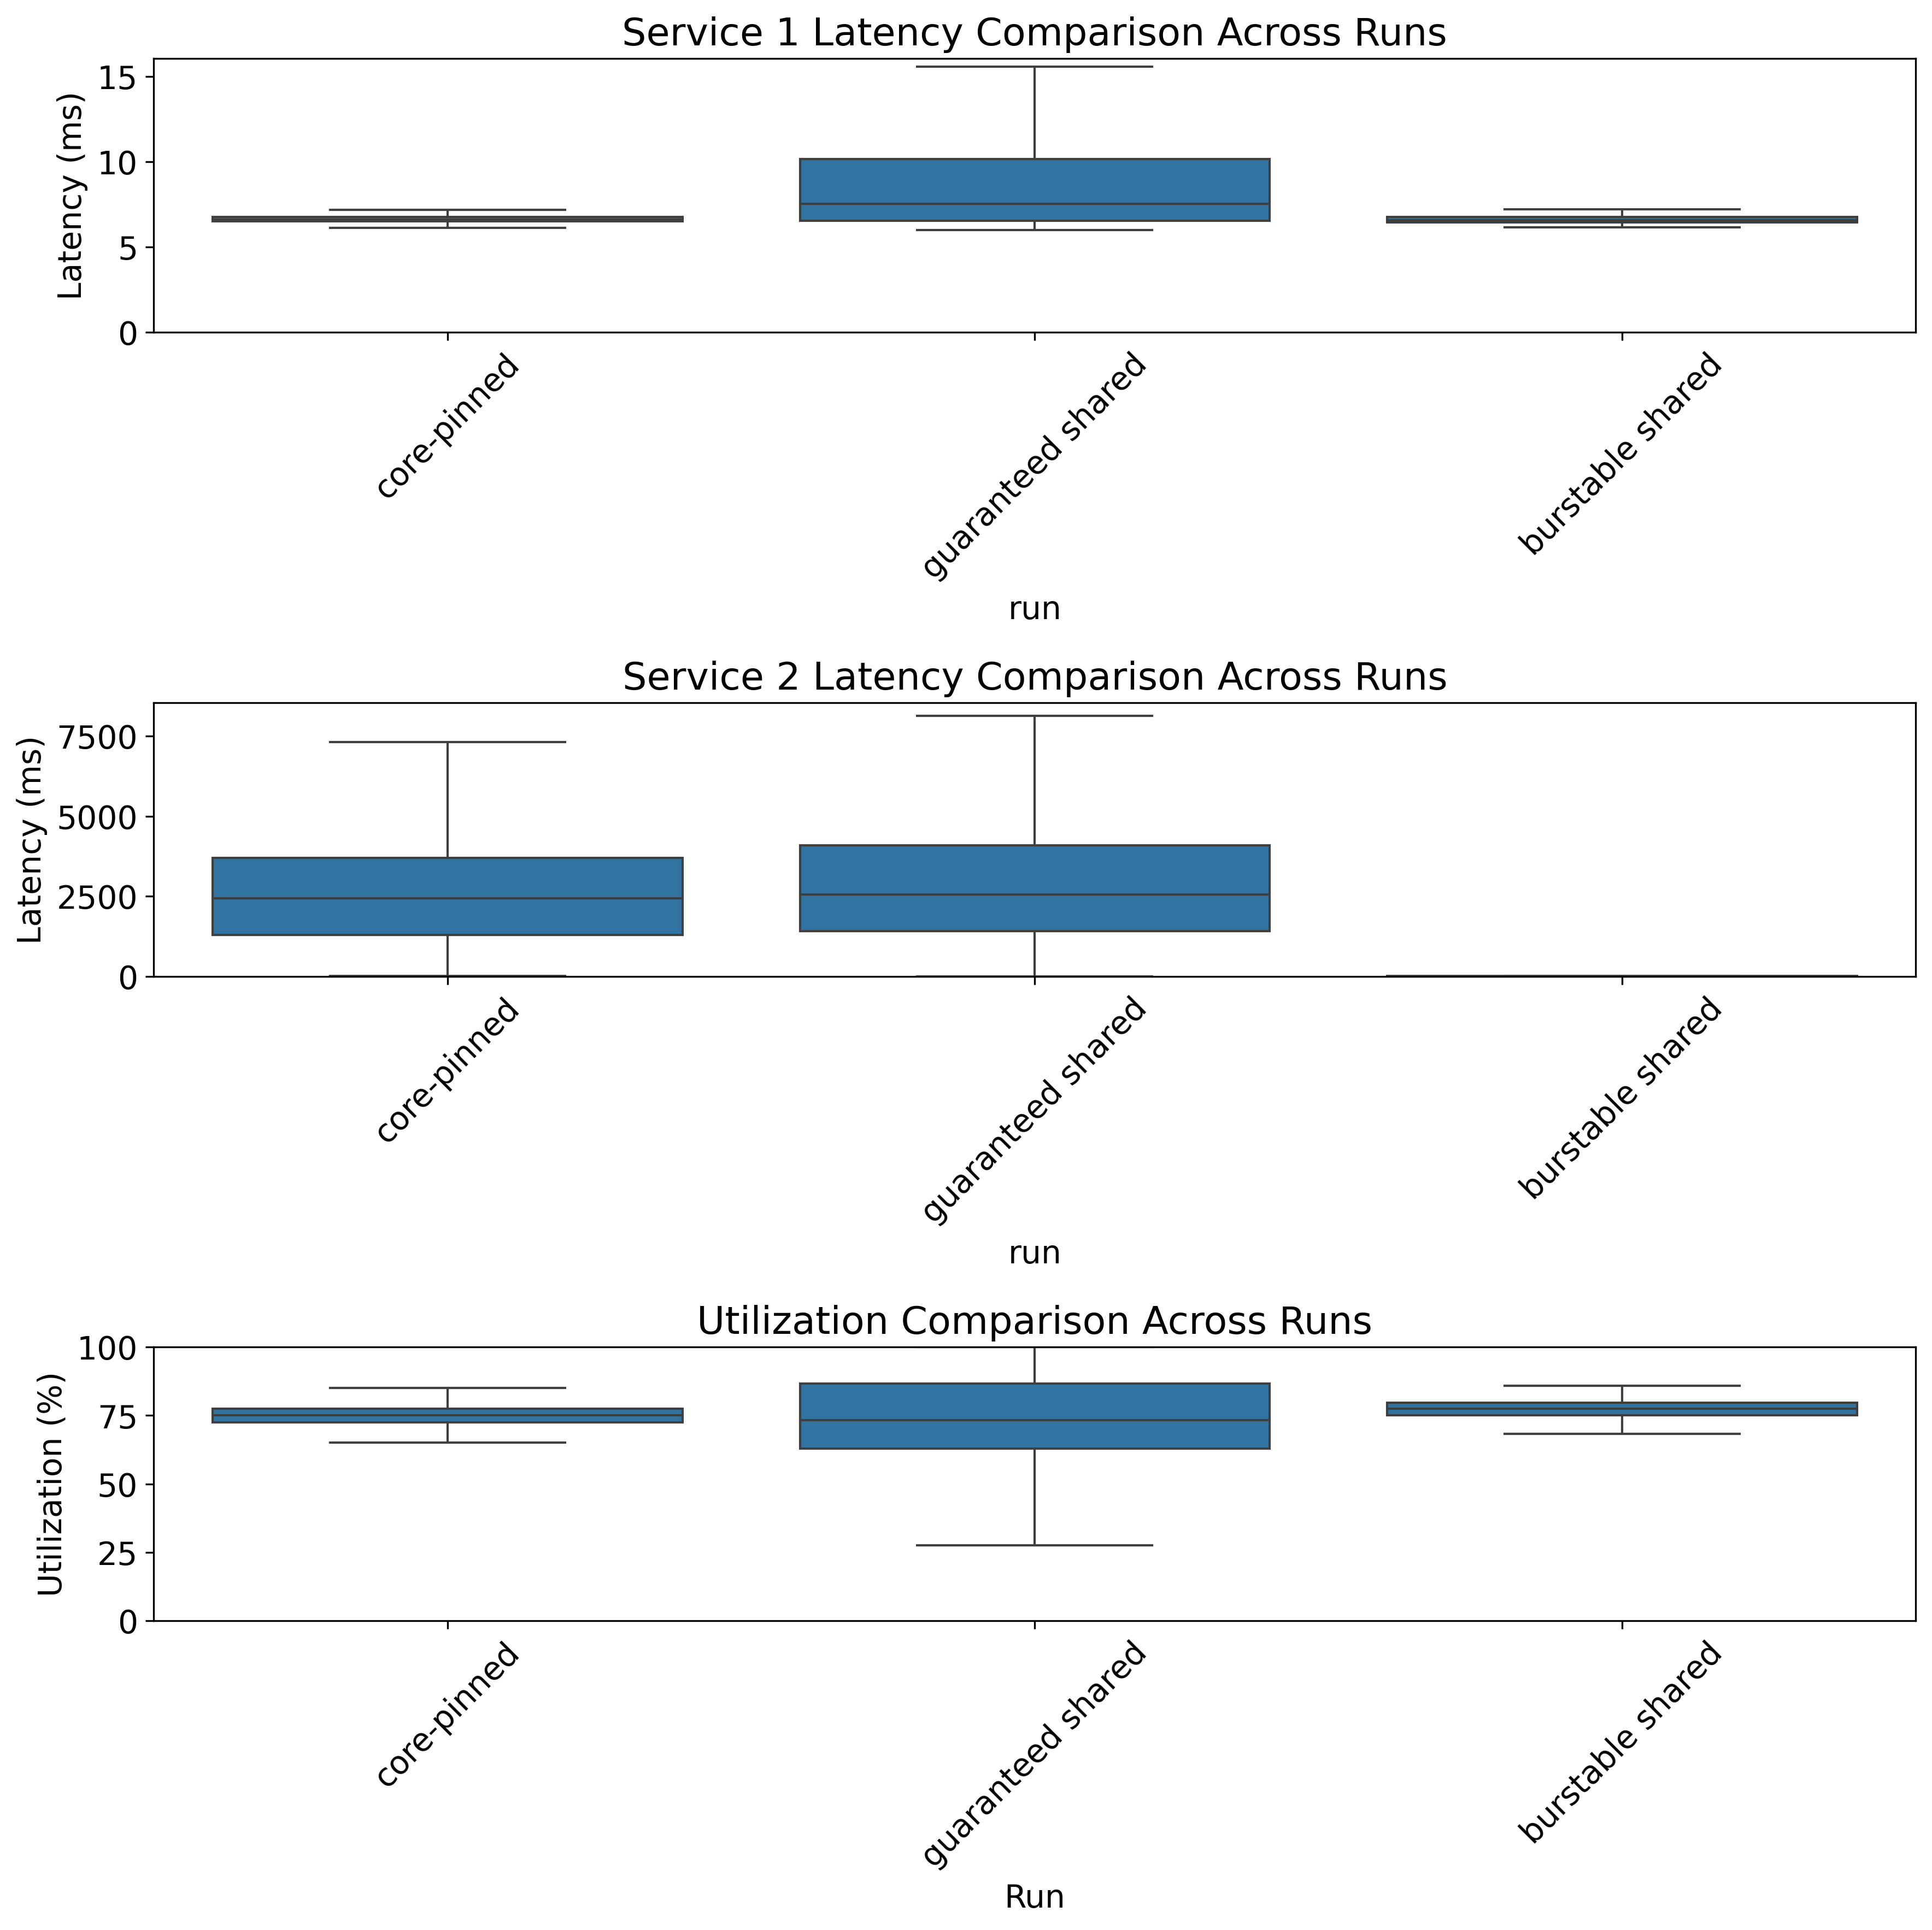
\includegraphics[width=\columnwidth]{graphs/kubernetes-lc-lc-cmp.png}
    \caption{In Kubernetes, running anything alongside a server in the
    Guaranteed QOS class affects the server's
    performance}\label{fig:kubernetes-qos-cmp}
\end{figure}

However, we find that current popular scheduling systems fail to properly
enforce reservations. We use as a case study a small but realistic social
network web application, which we run using Kubernetes.
\autoref{fig:kubernetes-qos-cmp} shows that running anything, even another
guaranteed service, alongside the web server affected its end-to-end latencies,
and that these effects go away when using core-pinning.\hmng{edited up to here}

Understanding why Kubernetes fails to honor the web application's reservation
requires looking at the underlying mechanism enforcing the CPU reservation:
Linux's \cgroups{}. In fact, most modern containers rely on \cgroups{} for CPU
isolation: all Open Container Initiative (OCI) compliant containers, including
Kubernetes but also Docker, CRI-O, and containerd
do~\cite{oci-cgroups,docker-docs-cgroups,container-isolation-article}. VM
frameworks, including Firecracker, AFaas and libvirt, also rely on \cgroups{} to
manage CPU time reservation~\cite{firecracker-cgroups,afaas,libvirt-cgroups}.

Weight is the part of the \cgroups{} interface these systems use for enforcing
the reservations LC applications have, while still allowing BEs without
reservations to run opportunistically.\footnote{Other operating systems expose a
similar interface, for instance Windows exposes a number of shares.} Kubernetes
creates one top level group for all best effort services, called
\texttt{kubepods-besteffort}, inside which all BE pods are placed, and assigns
it the lowest possible weight of 1. Pods with reservations are separated into
Burstable and Guaranteed, the main difference being that Guaranteed pods require
a limit to be set on the resources it can use. Kubernetes calculates the weight
that each pod gets based on the amount of milliCPUs it requests. For instance,
in the \autoref{fig:kubernetes-unedited} experiment, the web application service
ran in the Guaranteed class and asked for 4 CPUs, and Kubernetes assigned the
underlying pod a weight of 157.

The \cgroups{} documentation specifies that each group should get CPU time
proportional to its weight as a share of the sum of weights of runnable
groups~\cite{cgroups-kerneldocs}. However, the latency increase we see after
starting the best effort tasks in \autoref{fig:kubernetes-unedited} is much more
than the 1\% CPU time the server should be losing out on based on its weight. As
we show in more detail in \autoref{s:problem}, the problem that leads to the
increased latencies observed is that Linux will run a low weight process on one
core, unaware that a high weight process is runnable and waiting on another.
This happens because Linux uses per-CPU runqueues, which avoids the overheads of
having a global runqueue. A key challenge this work addresses is managing this
tension between how often the scheduler has to look at all the other cores'
runqueues to enforce reserved processes' priority globally, while still running
best effort ones opportunistically.

Our approach addresses this challenge by creating a new priority class for best
effort tasks to run in, \beclass{}, and enforcing it in the scheduler via
priority scheduling. Linux already has other classes between which it enforces
strict priority, which are designed and used for real time applications
(\autoref{ss:approach:linux-classes-isolate}); the proposed \beclass{} sits
below the default scheduling class. As we show in
\autoref{ss:approach:solves-problems}, putting best effort processes in a
separate class from those with reservations makes it viable to enforce those
reservations across cores, because it reduces the number of times the scheduler
is required to look at all the other cores' runqueues. Enforcing weights across
cores requires the scheduler to do so every scheduling tick, but with a separate
class it only has to look at other cores on \textit{class boundary crossings}:
every time a core switches from running an LC process to running a BE on, and
every time it enqueues an LC process.

A challenge with creating a separate priority class arises when the LC class is
under high load: completely starving best effort processes can lead to issues
such as deadlocks, broken TCP connections, or missed timers. The goal is to make
the priority of processes with reservations over those without as strict as
possible, while still allowing BE processes to resume execution normally once
the load goes down, even if the high load lasts for multiple minutes.

We address this challenge by enabling best effort processes to exist in an
ephemeral state called \textit{parked}, which they enter when the CPU
utilization is high enough that processes with a reservation account for all the
CPU time. While load remains high, the scheduler ensures that the parked BE's
user-space process doesn't run and consume resources, but continues to run the
kernel-space handlers that manage critical state, including TCP connections and
timers, on behalf of the BE processes. 

We implement \beclass{} in Linux on top of an existing scheduling policy called
\schedidle{}, and show that it is able to significiantly improve Linux's ability
to honor reservations while sharing CPUs with best effort workloads: in the same
Kubernetes experiment, the increase in average latency when starting a BE
workload goes from $>$2x to 0. The contributions of this paper are thus as
follows: 
\begin{enumerate}
    \item identifying as the reason LC tasks' reservations are often violated is
    that \cgroups{} does a poor job of enforcing the weights across cores;
    \item the design of \beclass{}, a new class for best effort tasks whose goal
    is to enforce reservations in the presence of BE processes by using priority
    scheduling, that reduces the points in time it needs to look at other core's
    runqueues, as well as enforcing the parked state
    \item an implementation of \beclass{} in Linux
\end{enumerate}



\section{Why}
\label{sec:why}

In order to understand why this is happening, we examine a trace of the
experiment. We use schedviz~\cite{schedviz}, a tool that visualizes perf traces,
to examine the scheduling decisions Linux is making.

\begin{figure*}[t]
    \centering
    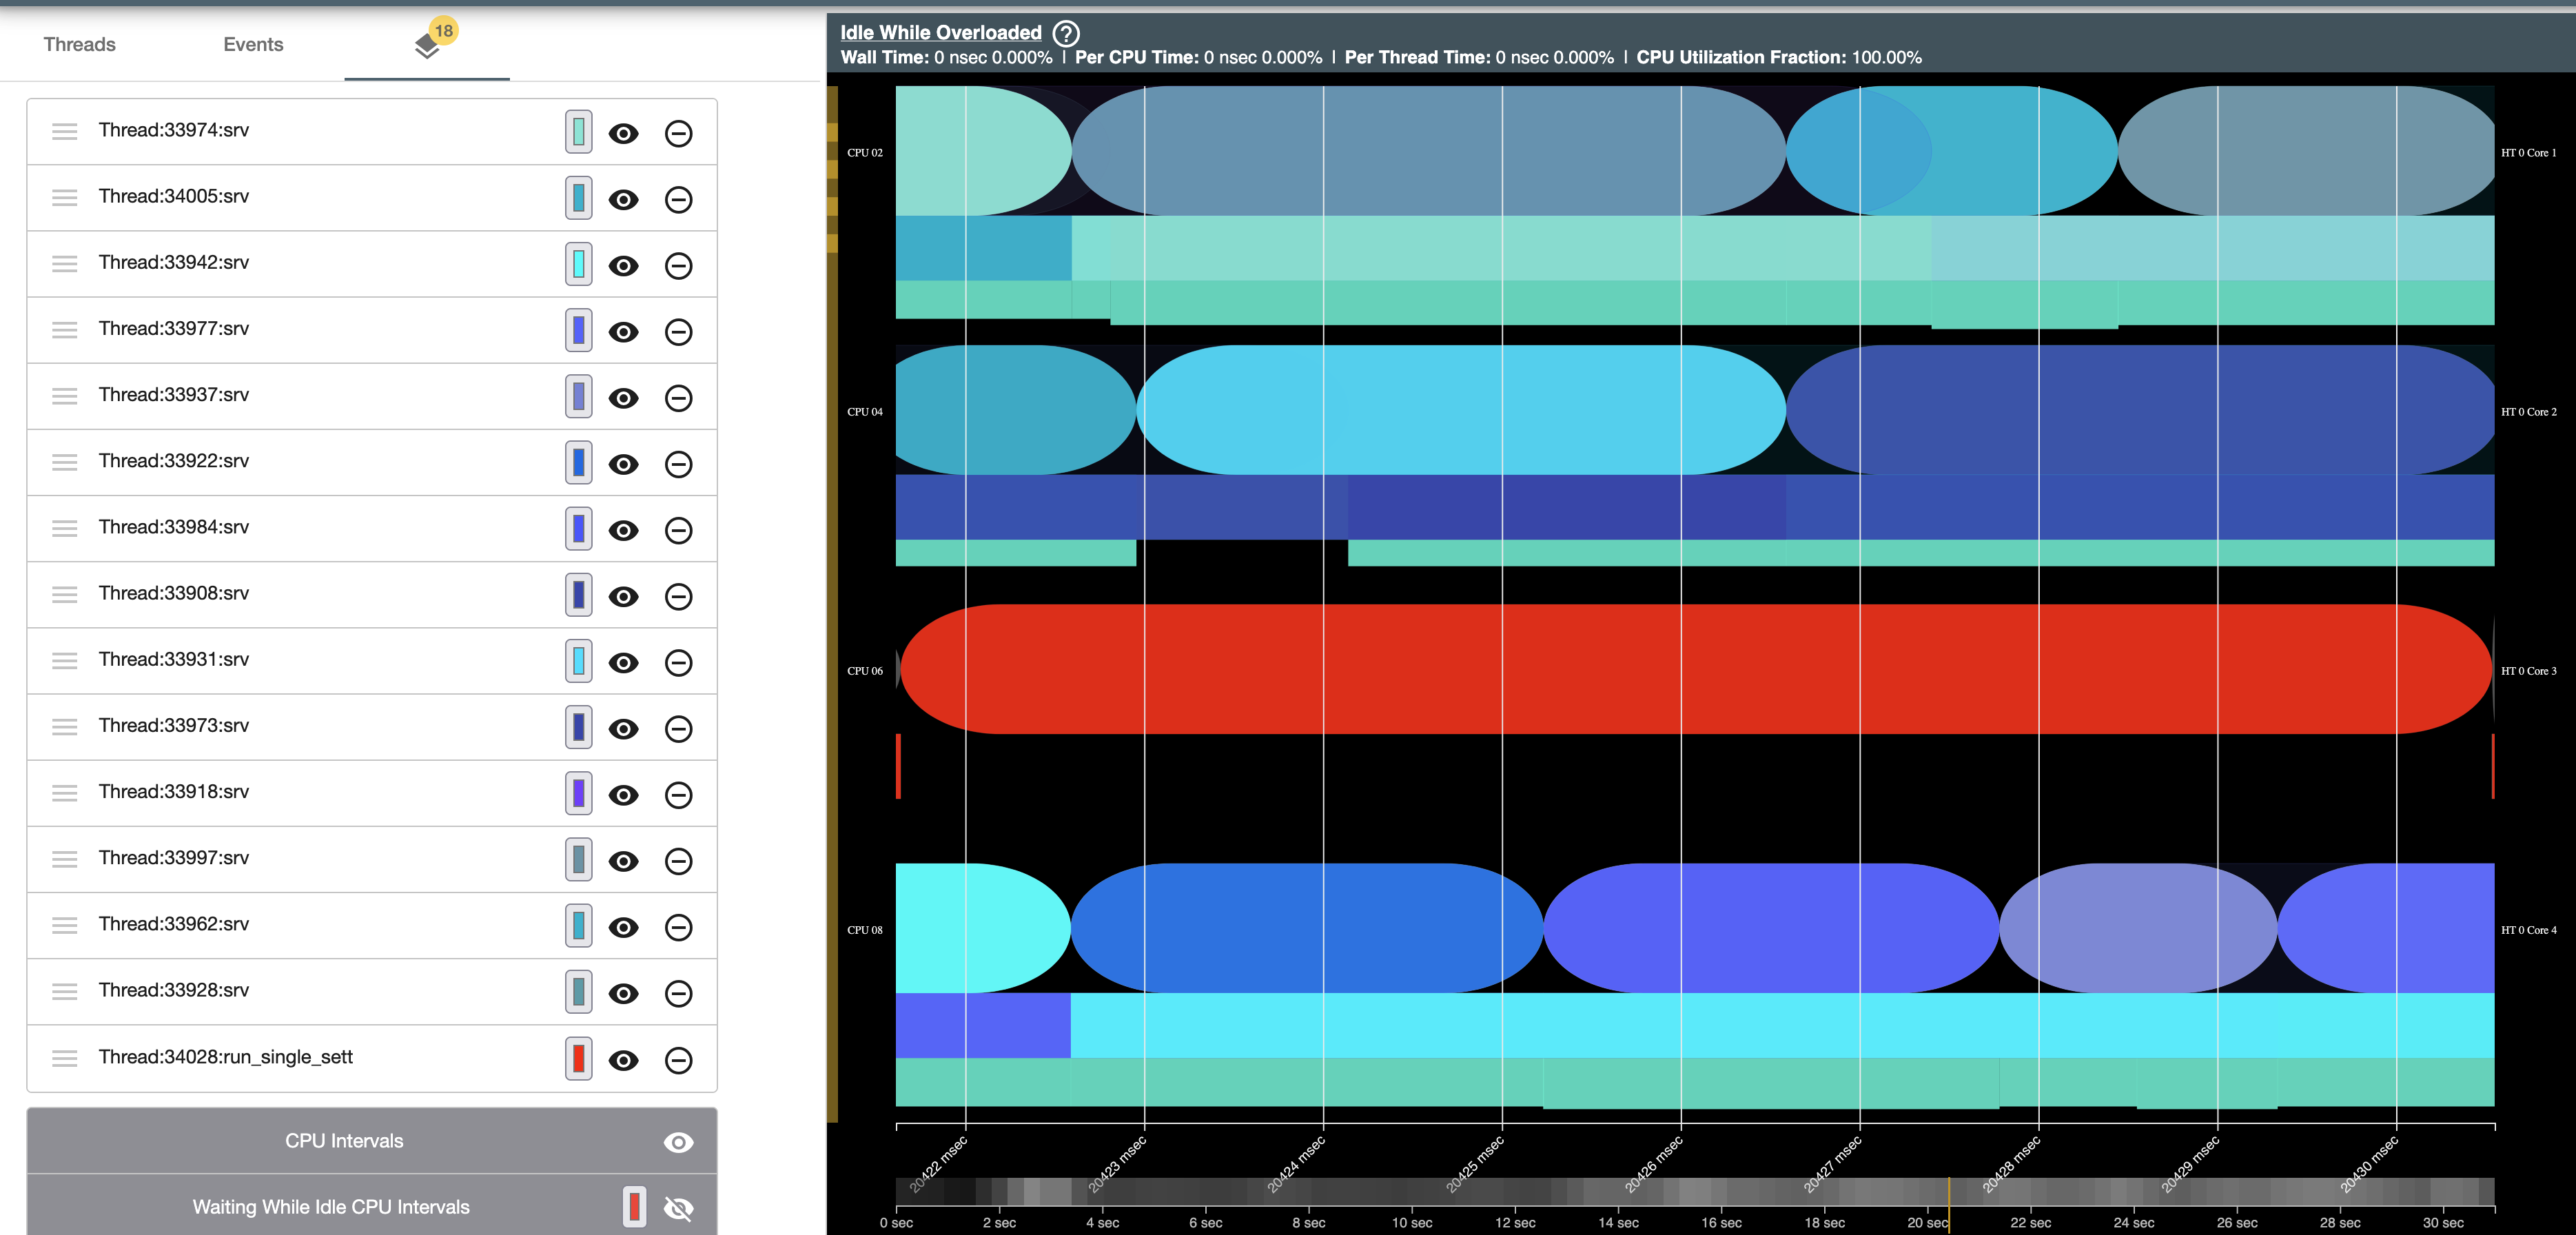
\includegraphics[width=\textwidth]{graphs/schedviz.png}
        \caption{Each thread is a different color. Circles represent which
    thread is running on that core, while rectangles underneath show waiting but
    runnable threads. Core numbers are 2,4,6,8 because this was run on a NUMA
    node so those are the cores that are closest to each other
    }\label{fig:schedviz}
\end{figure*}

In figure~\ref{fig:schedviz}, we look at a 10ms outtake from one of the runs,
that shows the problem occurring. The undesirable behavior we see here is that,
on core 6, the red process that is running the whole time is a BE process. All
the active server threads, shown in varying shades of blue, are on the other
cores, running and, more importantly, waiting.

The reason this happens is that Linux maintains a separate runqueue on each
core. This avoids the synchronization overheads of accessing global state for
every scheduling, but also means that the weight is only strictly enforced
within the individual runqueues, ie within each core. This leads to the depicted
failure mode, where an LC task is waiting on one core while another runs a BE
task.

% \hmng{should I also mention the giving at minimum 4ms? and how that can impact
%  tail latency}



\section{Real time scheduling}
\label{sec:sched-rt}

There is a way to configure tasks so that Linux enforces global priorities:
processes that run in real time have strict priority over other processes, and
are under a different scheduler that enforces strict and global priorities among
the real time threads.

Linux implements real time scheduling alongside the usual weighted fair share by
supporting different \textit{scheduling classes}. There are three scheduling
classes that are accessible to users, listed in descending order of priority:
Deadline, Fifo, and Normal. Generally speaking most load is expected to fall
into the Normal scheduling class (hence the name). It is the default scheduling
class, and it is only within the Normal scheduling class that the cgroup
cpu.weight interface is relevant.

Each scheduling class exists completely separately: classes maintain their own
run queues and per-entity state; implement their own scheduling algorithms to
choose from the entities on their runqueue; and balance the load across
runqueues on different cores.

Linux isolates strictly between different scheduling classes: it only schedules
a lower scheduling class if the higher scheduling classes found nothing to run,
and each scheduling class tries to steal work from other cores before returning
that it has nothing to run. It is thereby true that if something in the Normal
scheduling class is running, it means there are no Fifo tasks waiting to run
anywhere on the machine.

\begin{figure*}[t]
    \centering
    \begin{subfigure}[t]{0.48\textwidth}
        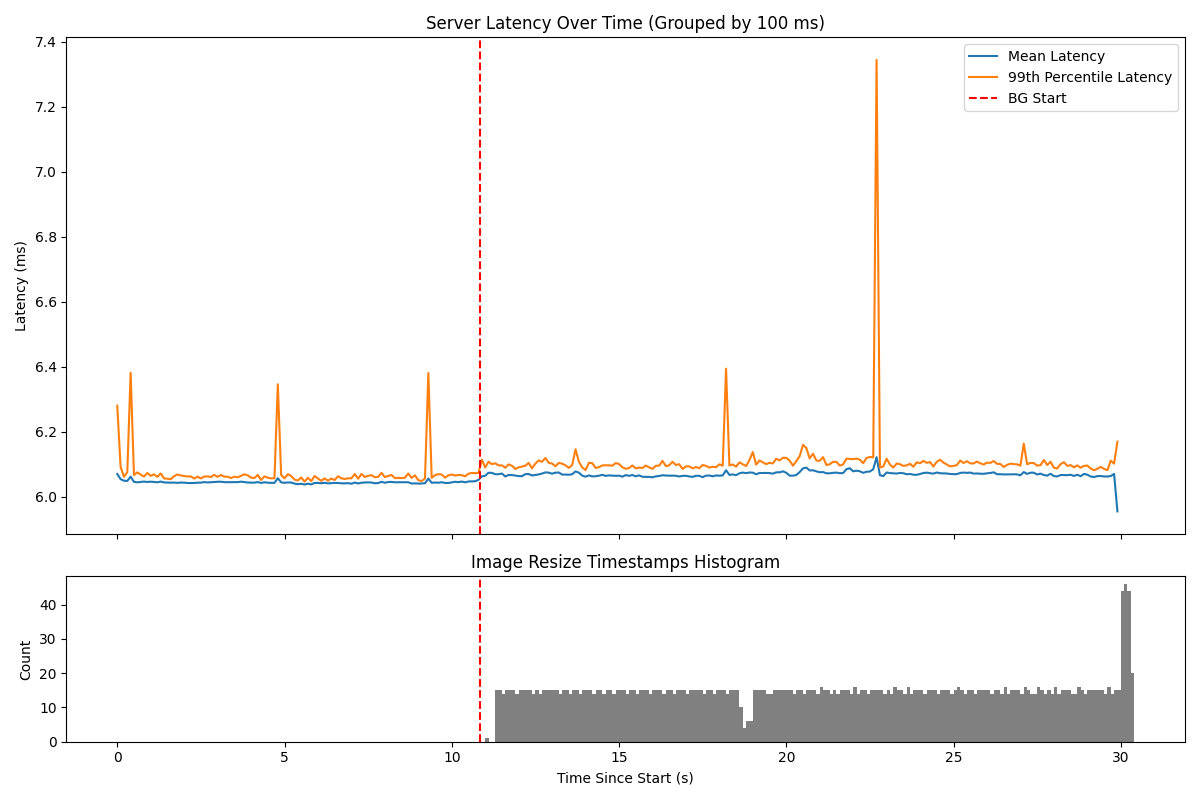
\includegraphics[width=\textwidth]{graphs/unedited-rt-low-two.png}
        \caption{Low load}\label{fig:unedited-rt-low-two}
    \end{subfigure}
    \hspace{\fill}
    \begin{subfigure}[t]{0.48\textwidth}
        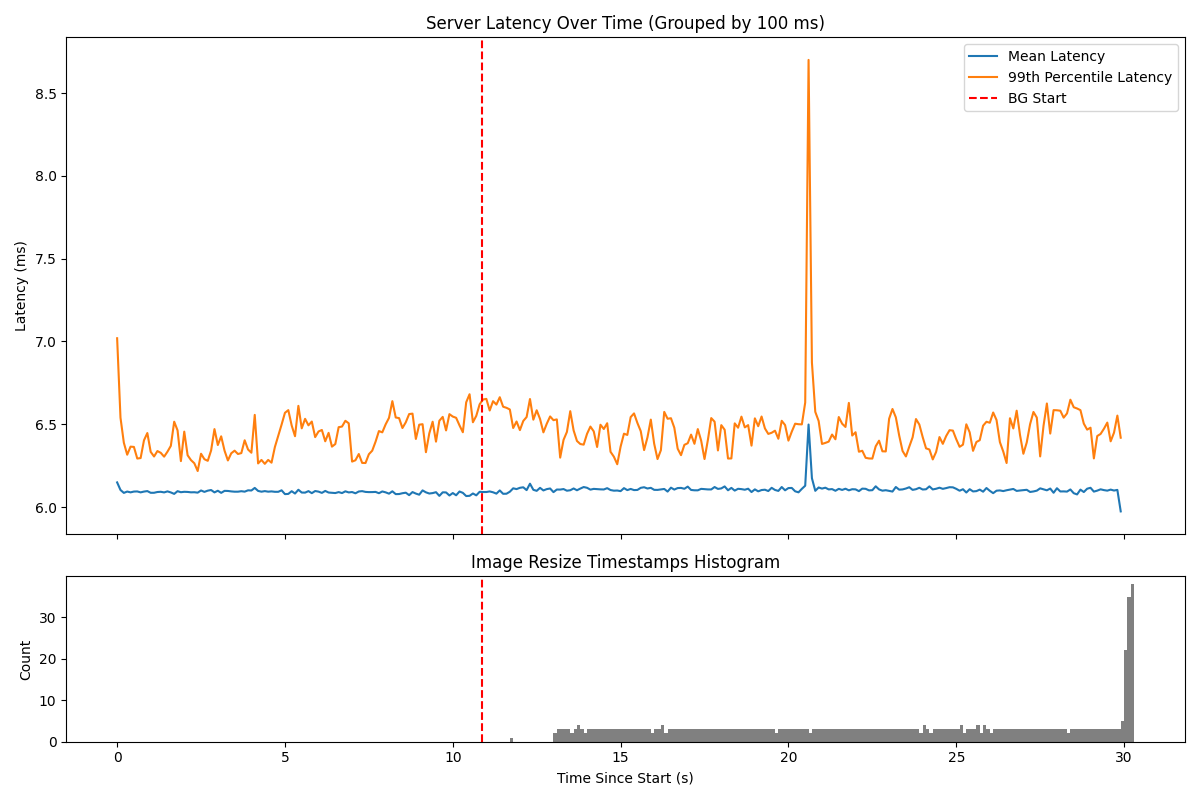
\includegraphics[width=\textwidth]{graphs/unedited-rt-high-two.png}
        \caption{High load}\label{fig:unedited-rt-high-two}
    \end{subfigure}
    \caption{Results of the same experiment, with LC running as a real time process}\label{fig:unedited-rt}
\end{figure*}

This points to a possible solution: run LC in Fifo and BE in Normal. Doing so
effectively promotes the latency criticality of the LC task in the eyes of the
system, and makes use of Linux's strong isolation of real time workloads.
Figure~\ref{fig:unedited-rt} shows the resulting measured latencies in the same
low and high load setting as previously. We see much stabler latencies, as
expected; in the baseline as well as once the BE tasks are started. This looks
promising on two fronts: 1: we get better isolation by making use of Linux's
strict boundaries between scheduling classes, and 2: we see improved tail
latency for the LC task by using a fifo run-to-completion scheduling algorithm.

However, the first benefit of improved stability comes at a cost. Because the
global ordering is so strict, also within the Fifo scheduling class, Linux is
performing balancing and potentially migration almost every time an LC thread
wakes up or exits. This requires the scheduling core to potentially lock the
runqueues of all the other cores as it ensures the task it will run the next is
the one with the highest priority, and within that priority the once that first
became runnable. This increase in scheduling latency leads to the small increase
in the baseline latency that is visible in the graphs.

And second benefit, the observed improved tail latency, is a side-effect of the
experimental setup, where each request does the exact same thing and processing
times are uniform. This is not true for a production environment, where request
processing times are variable and unknown. If a fifo run-to-completion scheduler
is used in that setting, it leads to HoL blocking, and thus to much worse tail
latencies for short requests.

We conclude that the Fifo scheduling class is not a good solution: although it
is able to globally ensure isolation between LC and BE tasks, its scheduling
time overheads and algorithm make in poorly suited for a production setting.






\section{Half a scheduling class}
\label{sec:sched-idle}

\hmng{transition??}
Within the Normal scheduling \textit{class}, Linux supports two different
scheduling \textit{policies}: \schednormal{} and \schedidle{}, where
\schednormal{} is the default. Under the hood, Linux keeps tasks in both
policies on the same runqueue, and they are all scheduled using the same
algorithm. Thus, \schedidle{} is in principle not very different from just being
a low-weight process: For most intents and purposes, \schedidle{} entities are
just entities with a predefined low weight (currently 3). There is, confusingly,
also and Idle scheduling \textit{class}, but that not accessible to userspace
and exists solely to manage the core's transition in and out of being actually
idle (ie running nothing).

The main way that \schedidle{} entities are special-cased from \schednormal{}
entities in the scheduler is during wakeup: in 2019 a patch to Linux added a
check where, when a \schednormal{} entity becomes newly runnable, if the core
where the entity is waking up is already running something in \schednormal{}, it
will look for other cores that might be currently running a \schedidle{} entity,
and migrates the new entity there.

In doing so, Linux created a half scheduling class. In order to implement fully
invariant that no process of category B is ever running if a task of category A
is queued, that requires 1: checking if other cores are running a B task when an
A task wakes up on a core already running an A task, and 2: checking if another
core has a queued A task before running a B task.\ \schedidle{} does step 1, but
not step 2.

\schedidle{} is also promising because it was extended to have cgroup support
recently: when set via the cpu.idle cgroup interface file, the entire cgroup is
counted as a \schedidle{} entity.

\begin{figure*}[t]
    \centering
    \begin{subfigure}[t]{0.48\textwidth}
        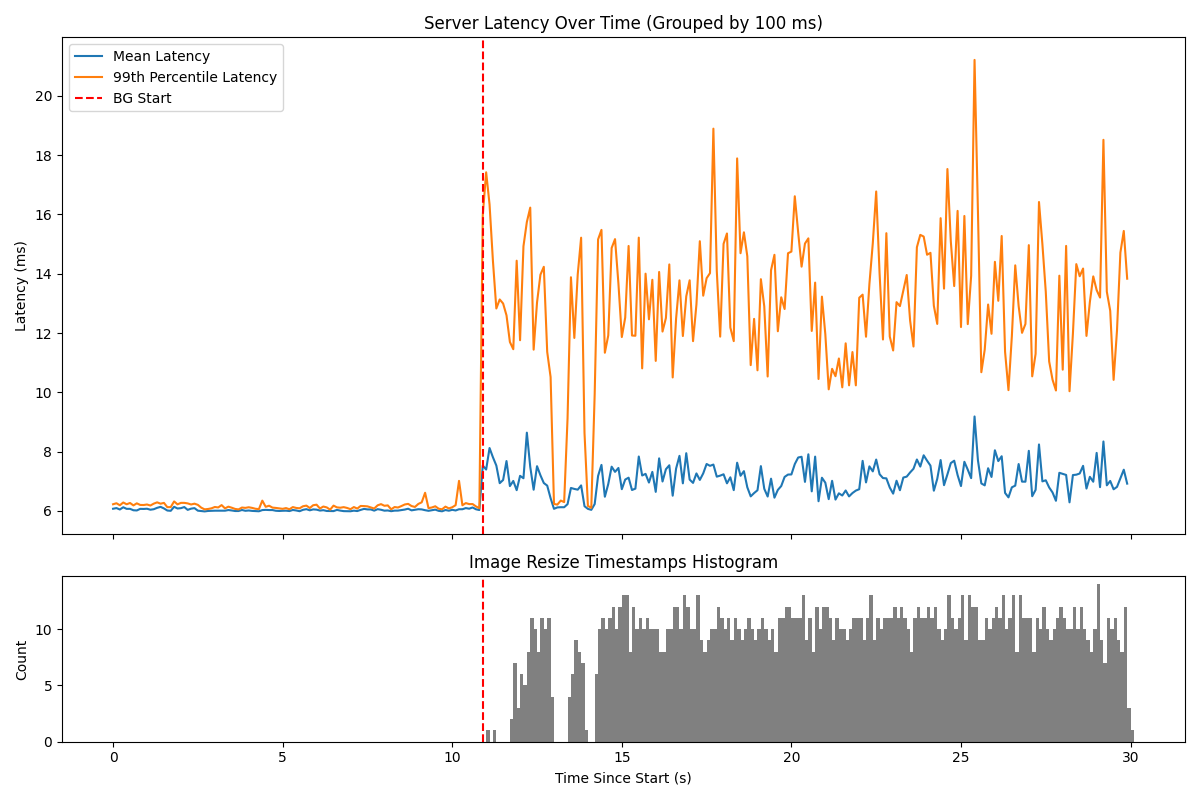
\includegraphics[width=\textwidth]{graphs/unedited-idle-low-two.png}
        \caption{Low load}\label{fig:unedited-idle-low-two}
    \end{subfigure}
    \hspace{\fill}
    \begin{subfigure}[t]{0.48\textwidth}
        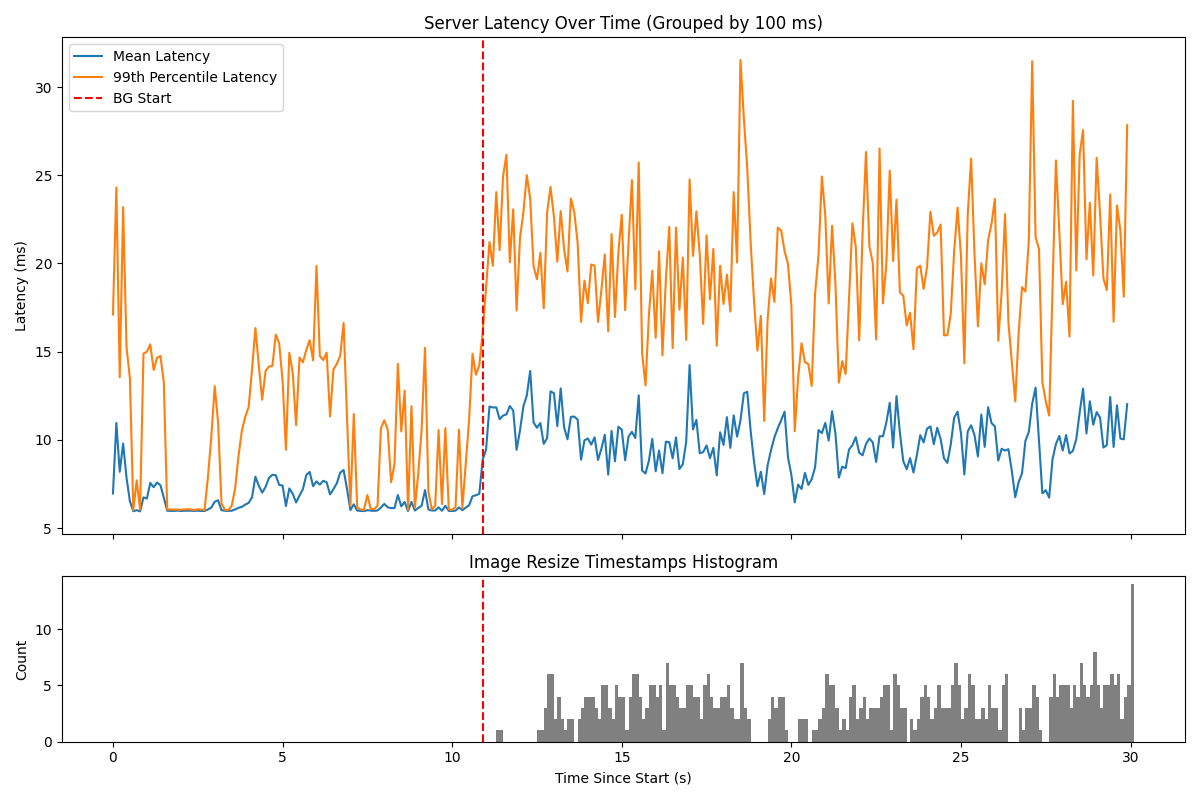
\includegraphics[width=\textwidth]{graphs/unedited-idle-high-two.png}
        \caption{High load}\label{fig:unedited-idle-high-two}
    \end{subfigure}
    \caption{using \schedidle{}}\label{fig:unedited-idle}
\end{figure*}

And indeed, we find that when we use cgroups' new cpu.idle interface feature,
the latency impact of the BE tasks decreases, although it does not entirely drop
to what we saw with the Fifo class. Figure~\ref{fig:unedited-idle} shows the
results, for the familiar settings of low and high load. The jump we see in the
mean latency has decreased from peaks as high as 13ms to around 7ms (even though
in principle they now have a higher weight).





\section{Making it whole}
\label{sec:my-patch}

The performance of the current \schedidle{} policy shows us that if we want to
completely isolate LC and BE, we need to put in the final piece to make
\schedidle{} effectively its own scheduling class.

We write a Linux patch that does this. The patch intervenes in two places in the
current scheduling process: 1: it ensures that no \schedidle{} entity will be
chosen if there is a runnable \schednormal{} entity (this overrides the fair
share that even a weight 1 process would occasionally get in unmodified kernel),
and 2: it tries to steal queued \schednormal{} entities from other cores before
running a \schedidle{} entity.

\begin{figure*}[t]
    \centering
    \begin{subfigure}[t]{0.48\textwidth}
        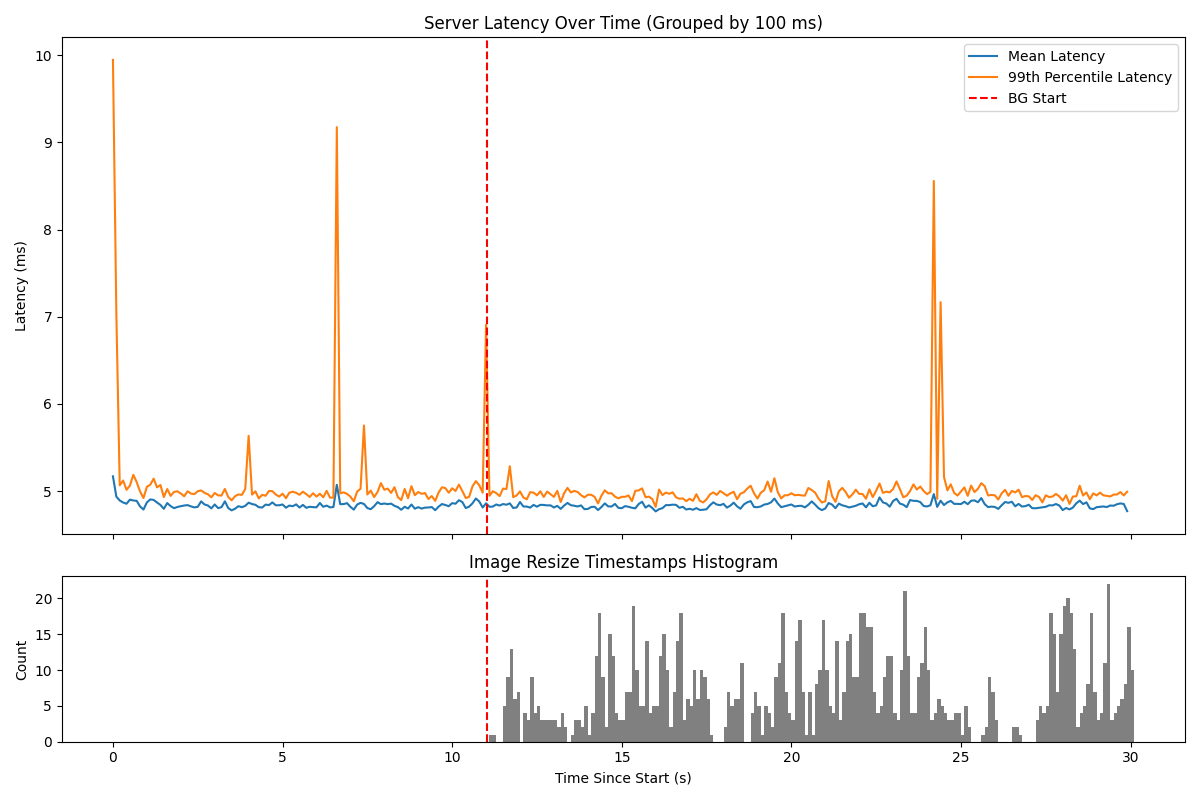
\includegraphics[width=\textwidth]{graphs/patched-idle-low-two.png}
        \caption{Low load}\label{fig:patched-idle-low-two}
    \end{subfigure}
    \hspace{\fill}
    \begin{subfigure}[t]{0.48\textwidth}
        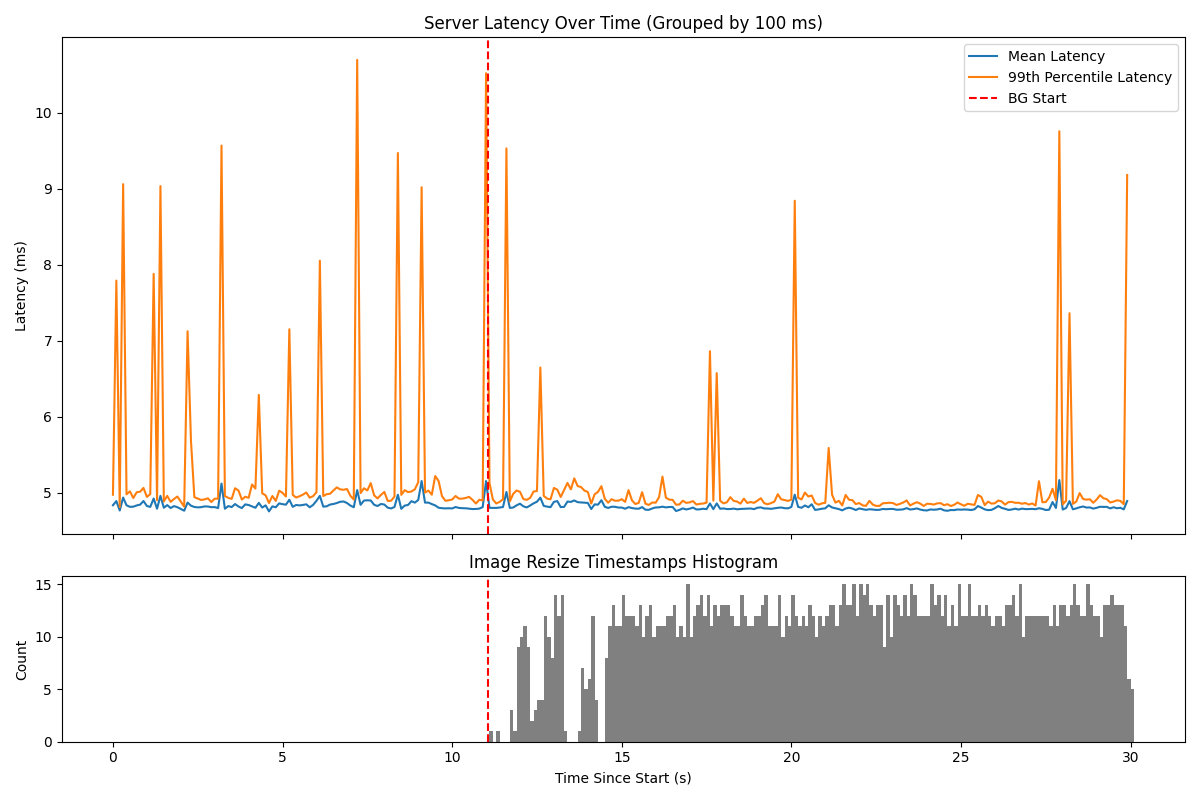
\includegraphics[width=\textwidth]{graphs/patched-idle-high-two.png}
        \caption{High load}\label{fig:patched-idle-high-two}
    \end{subfigure}
    \caption{using a patched \schedidle{} that steals queued \schednormal{}
    tasks before running \schedidle{} ones}\label{fig:patched-idle}
\end{figure*}

We can see the resulting performance in figure~\ref{fig:patched-idle}, and see
that as desired the latency of the server remains stable after the background
tasks start. This does not mean that the background task never runs: the lower
graph still shows iterations of image resizing being done. The difference is
that now the background tasks will reliably get interrupted when the LC server
has a request to process.



%!TeX root = SM_Thesis_Proposal.tex

\section{Timeline}
\label{sec:timeline}

\textbf{1. Current state of the project:} 
The driving problem that motivated the project was multiple experiences of
confusing performance results in other projects, which pointed to a gap between
expectation and reality of Linux's cgroup interface. 

We have done a comprehensive analysis of the problem at different levels, by
looking at Linux's scheduling code as well as running many benchmarks and
profiling traces. This has allowed us to narrow down the problem to a simple
case that exhibits the undesirable behavior, and to be able to point to what
goes wrong, both in the traces and in the code.

We have experimented with different solution approaches, and landed on one that
requires editing the Linux migration code during scheduling decisions. We are
now at a point where we have a patch that leads to the desired behavior, and
have shown that it solves the simple case that we initially narrowed the problem
down to.

\textbf{2. Steps remaining:} In the time between now and the deadline, we plan
to further understand and push the solution. This includes three main
dimensions: we want to measure the exact costs (how long does the added code
take to run); we want to understand its implications (do things break when BE
processes are starved for longer periods of time); and finally we want to create
more realistic and end-to-end scenarios to understand the practical implications
of the change we made.

\textbf{2.a Measure the cost:} We plan to run a small microbenchmark where we
trigger the new patch code by running three \schednormal{} tasks and one
\schedidle{} task on two cores. We know the kernel will, once the \schednormal{}
task that has a core to itself completes, steal one of the others. We can use
that opportunity to measure how long it takes to run the code in the worst case
scenario, ie when it has to check the load and then also actually go and steal work.

\textbf{2.b Understand the implications:} Linux has many mechanisms to avoid
starvation of processes, and the change we make allows for starvation. We will
test this by starving a complex BE task (ie one that has open TCP connections,
files, etc) for a long period of time and ensuring that it can still continue
running as normal after.

\textbf{2.c End to end scenario:} The initial problem came from more complex
examples of more realistic applications than what we ended up reducing it to, so
we want to take the solution and apply it to these settings and demonstrate that
it improves performance as expected.




\bibliographystyle{plain}
\bibliography{references}

\end{document}
